\documentclass[12pt,letterpaper]{article}
\usepackage[utf8]{inputenc}
\usepackage[spanish]{babel}
\usepackage{graphicx}
\usepackage[left=2cm,right=2cm,top=2cm,bottom=2cm]{geometry}
\usepackage{graphicx} % figuras
% \usepackage{subfigure} % subfiguras
\usepackage{float} % para usar [H]
\usepackage{amsmath}
%\usepackage{txfonts}
\usepackage{stackrel} 
\usepackage{multirow}
\usepackage{enumerate} % enumerados
\renewcommand{\labelitemi}{$-$}
\renewcommand{\labelitemii}{$\cdot$}
% \author{}
% \title{Caratula}
\begin{document}

% Fancy Header and Footer
% \usepackage{fancyhdr}
% \pagestyle{fancy}
% \cfoot{}
% \rfoot{\thepage}
%

% \usepackage[hidelinks]{hyperref} % CREA HYPERVINCULOS EN INDICE

% \author{}
\title{Caratula}

\begin{titlepage}
\begin{center}
\large{UNIVERSIDAD PRIVADA DE TACNA}\\
\vspace*{-0.025in}
\begin{figure}[htb]
\begin{center}

\includegraphics[width=8cm]{./Imagenes/logo}
\end{center}
\end{figure}
\vspace*{0.15in}
INGENIERIA DE SISTEMAS  \\

\vspace*{0.5in}
\begin{large}
TITULO:\\
\end{large}

\vspace*{0.1in}
\begin{Large}
\textbf{INFORME DE LABORATORIO N5 - BI} \\
\end{Large}

\vspace*{0.3in}
\begin{Large}
\textbf{CURSO:} \\
\end{Large}

\vspace*{0.1in}
\begin{large}
INTELIGENCIA DE NEGOCIOS\\
\end{large}

\vspace*{0.3in}
\begin{Large}
\textbf{DOCENTE(ING):} \\
\end{Large}

\vspace*{0.1in}
\begin{large}
 Patrick Cuadros Quiroga\\
\end{large}

\vspace*{0.2in}
\vspace*{0.1in}
\begin{large}
Estudiante: \\
\begin{flushleft}
Salamanca Contreras, Fiorella Rosmery 		\hfill	(2015053237) \\
\end{flushleft}
\end{large}
\end{center}

\end{titlepage}


\tableofcontents % INDICE
\thispagestyle{empty} % INDICE SIN NUMERO
\newpage
\setcounter{page}{1} % REINICIAR CONTADOR DE PAGINAS DESPUES DEL INDICE

\section{IMPORTACION, DATA FLOW, TRASLADO DE ARCHIVOS} 

IMPORTAR DATOS USANDO EL WIZARD Y Desarrollar mis primeros PAQUETEs DTSX\\
“REQUERIMIENTOS: SQL SERVER INTEGRATION SERVICES 2012R2, BD ADVENTURE WORK (OLTP Y DATAWAREHOUSE) y AdventureWorksLT2012”

\begin{itemize}
    \item \textbf{TAREA 1 - IMPORTACION DE DATOS USANDO EL WIZARD – SQL MANAGMENT}

- Crear una base de datos – BDTEST\\
- Importar Datos desde AdventureWorks\\

	\begin{center}
	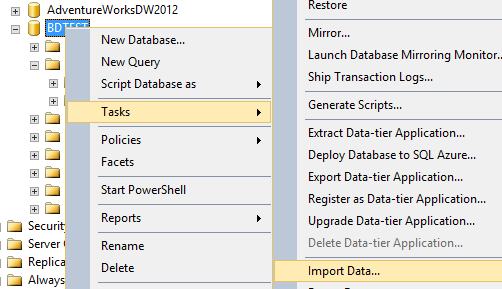
\includegraphics[width=12cm]{./Imagenes/1}
	\end{center}	

- Next y escribir el Servidor y seleccionar la base de datos

	\begin{center}
	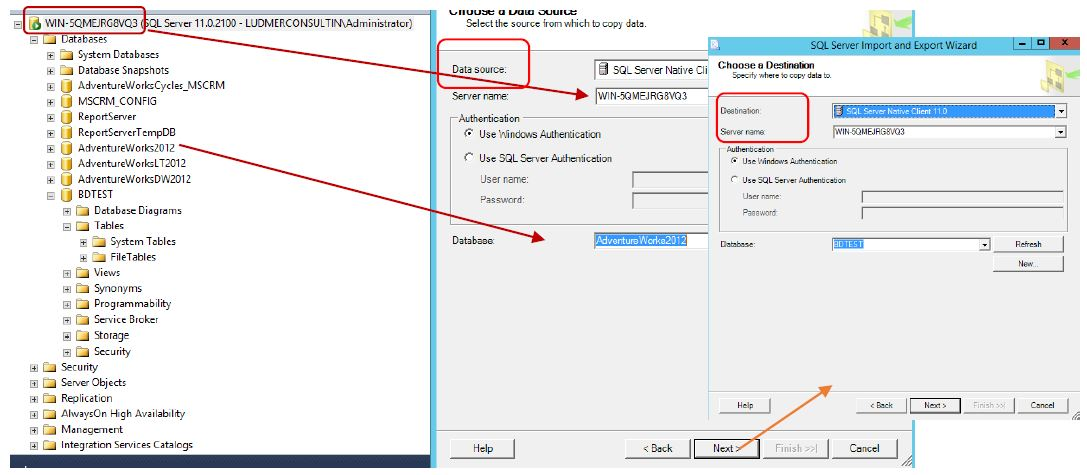
\includegraphics[width=17cm]{./Imagenes/2}
	\end{center}	

- Data Source: La base de donde vamos a importar\\
- Destination: La Base donde vamos a cargar la data

	\begin{center}
	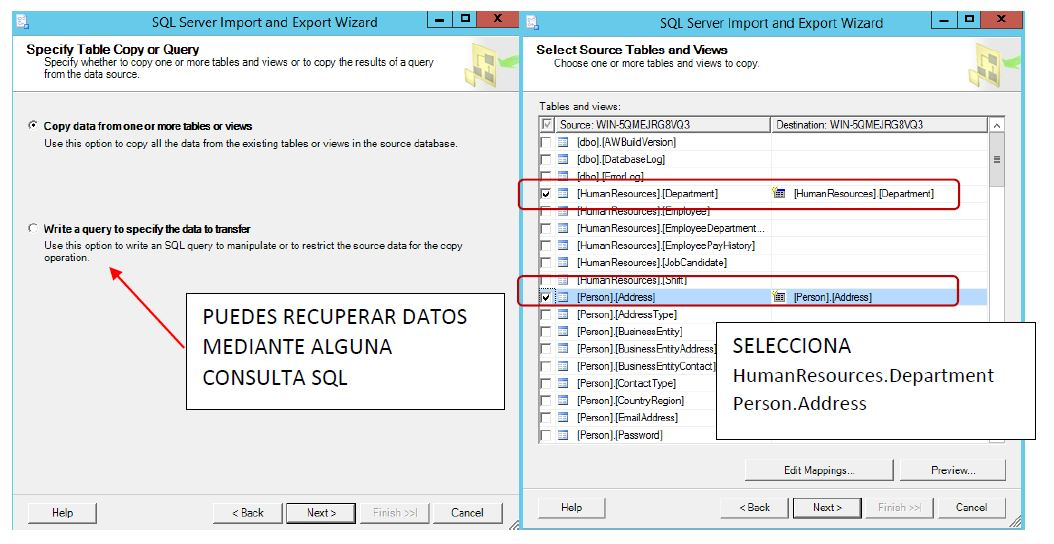
\includegraphics[width=17cm]{./Imagenes/3}
	\end{center}	

	\begin{center}
	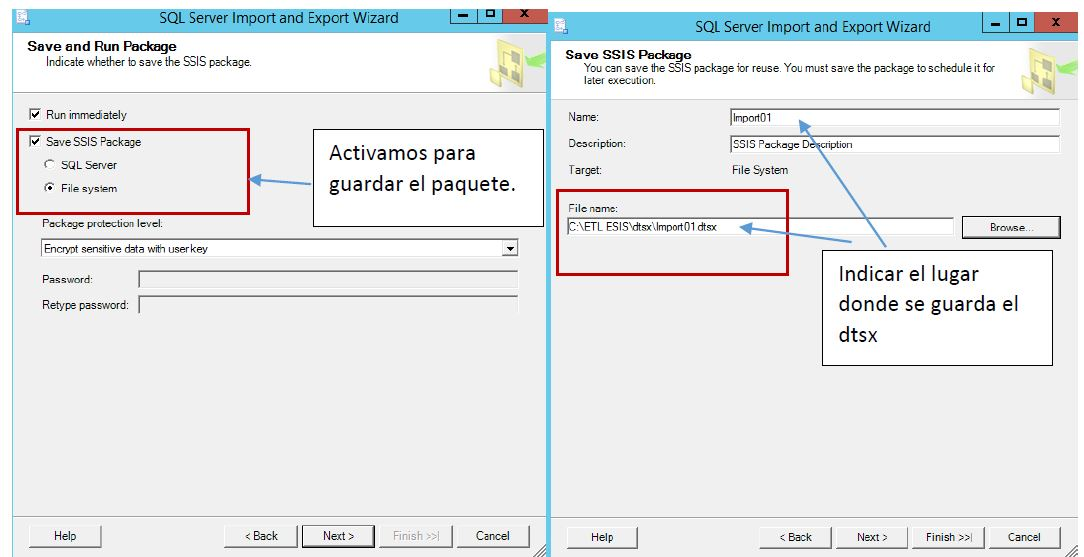
\includegraphics[width=17cm]{./Imagenes/4}
	\end{center}	

- AL Finalizar tenemos el resumen de la ejecución.\\
- HEMOS Generado nuestro 1 paquete de forma automatica.\\
- Podemos actualizar la base de datos\\
- BDTEST y encontraremos las tablas ya importadas.\\

	\begin{center}
	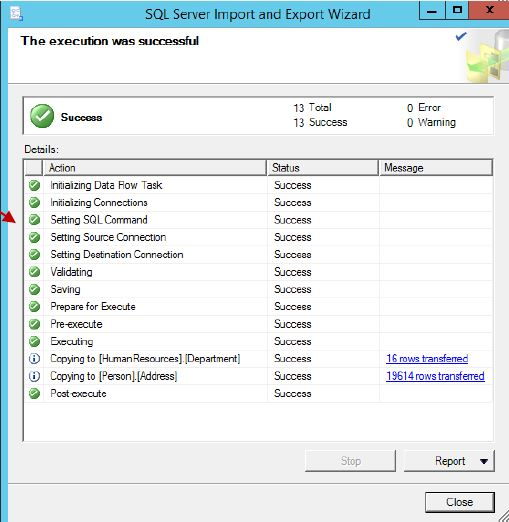
\includegraphics[width=14cm]{./Imagenes/5}
	\end{center}	

	\newpage

    \item \textbf{TAREA 2 - CREAMOS NUESTRO PRIMER PAQUETE DTSX}

	\begin{center}
	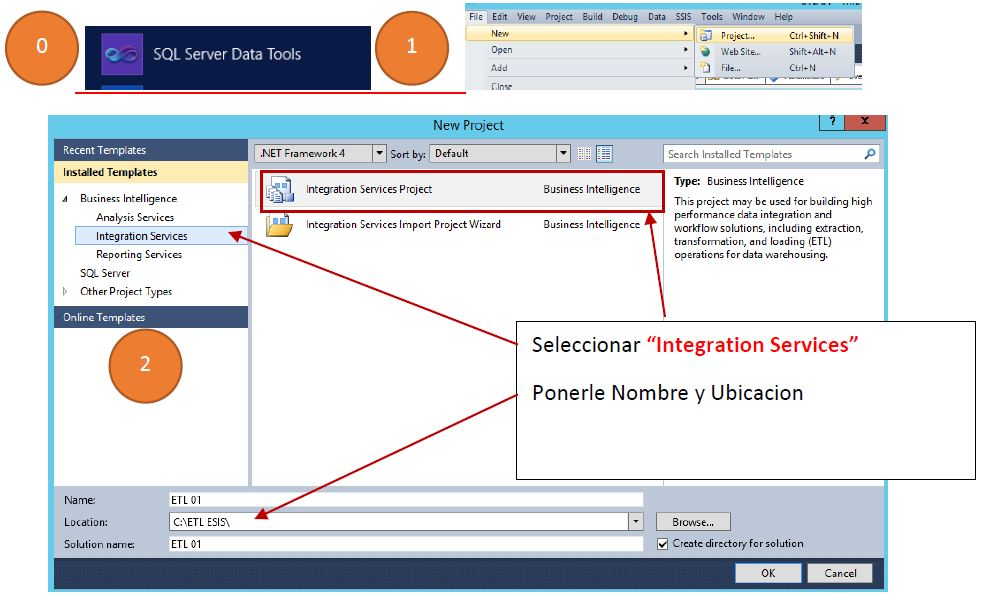
\includegraphics[width=17cm]{./Imagenes/6}
	\end{center}	

	\begin{center}
	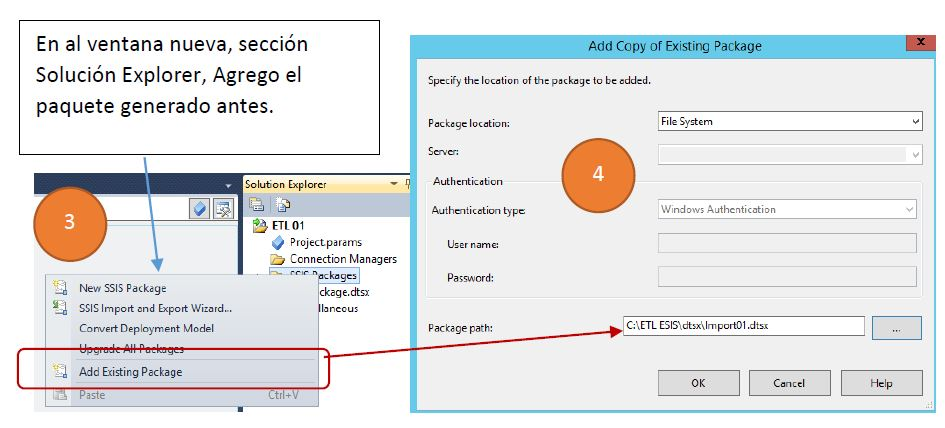
\includegraphics[width=17cm]{./Imagenes/7}
	\end{center}	

- LA SIGUIENTE VENTANA MUESTRA EL PAQUETE QUE SE HA IMPORTADO.

	\begin{center}
	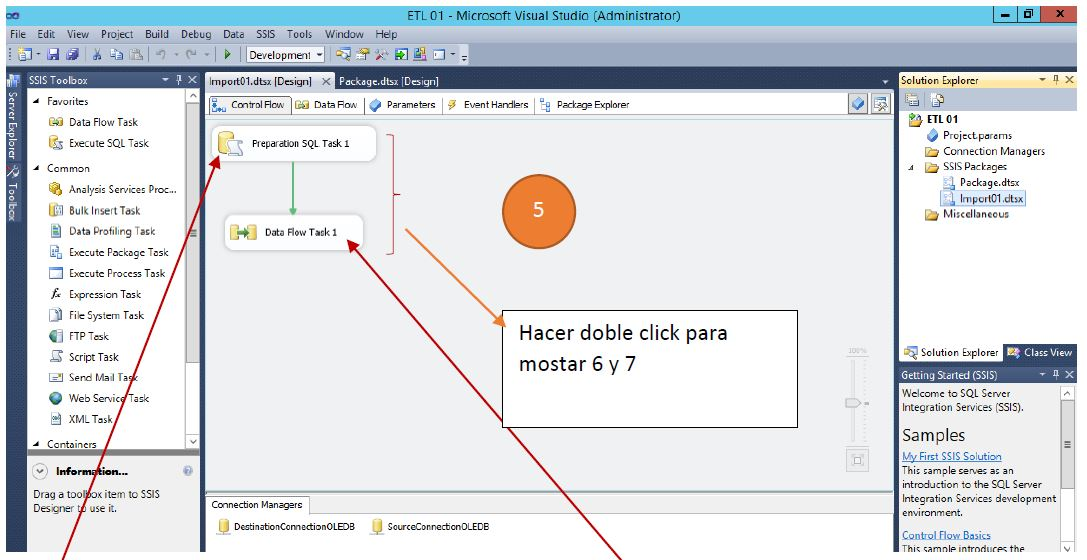
\includegraphics[width=17cm]{./Imagenes/8}
	\end{center}	

	\begin{center}
	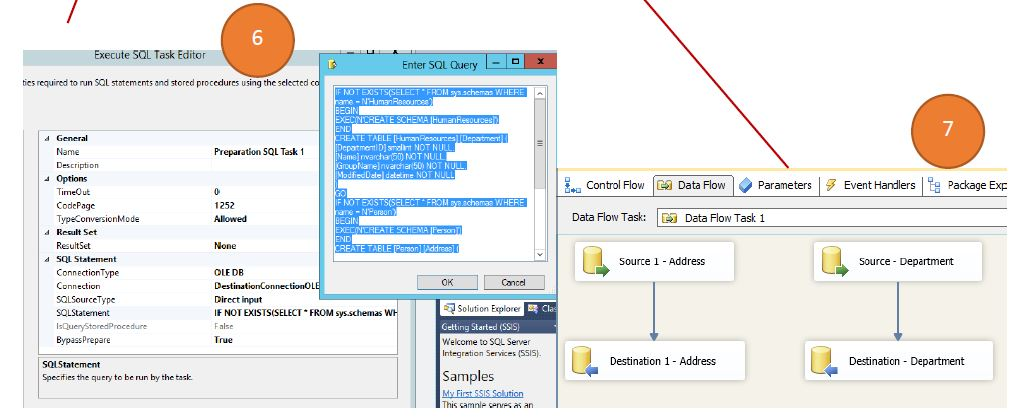
\includegraphics[width=17cm]{./Imagenes/9}
	\end{center}	
\end{itemize}
\section{PRESENTACION DEL ESPACIO DE TRABAJO} 

	\begin{center}
	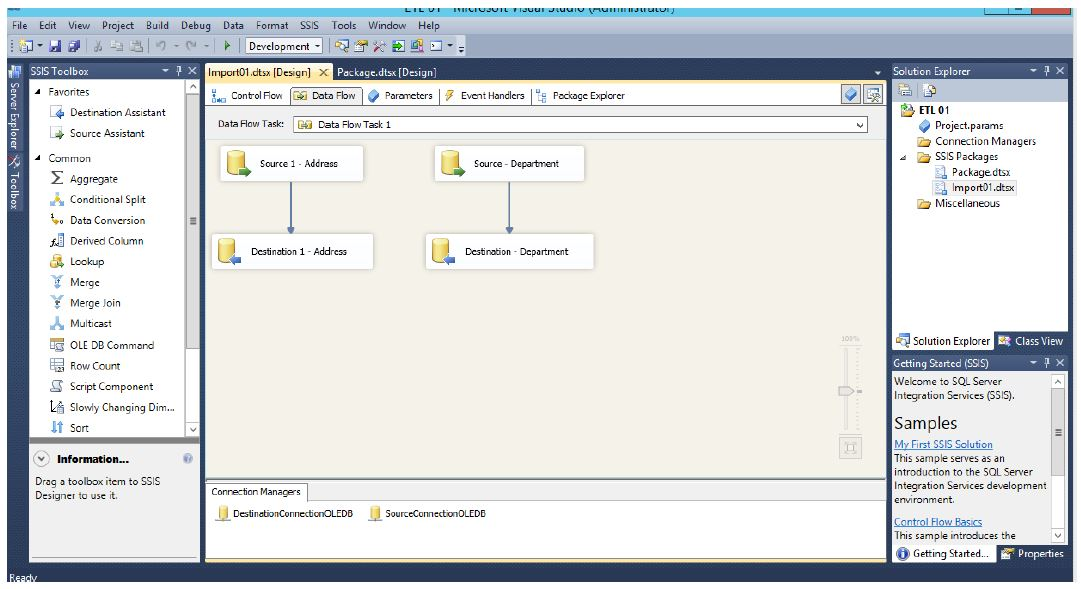
\includegraphics[width=15cm]{./Imagenes/10}
	\end{center}	

- MI PRIMER PAQUETE, Muestra la cantidad de Registros de una Tabla\\
- File - \textgreater NewProject - \textgreater

	\begin{center}
	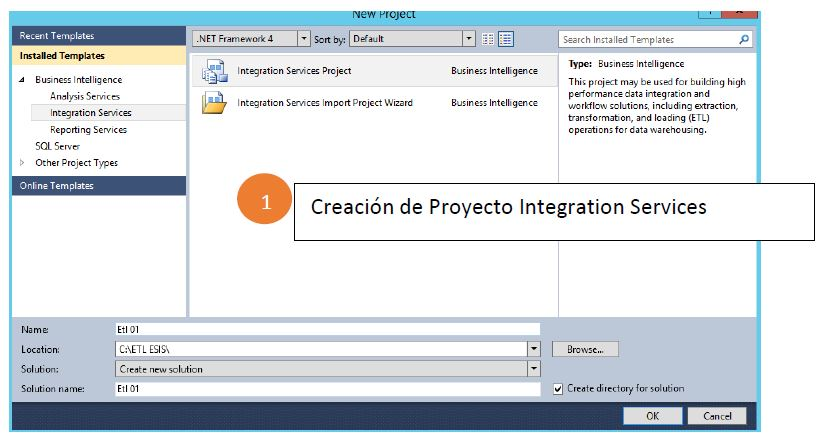
\includegraphics[width=15cm]{./Imagenes/11}
	\end{center}	

2. Creacion una conexión OLEDB para la base de datos Adventure Work.

	\begin{center}
	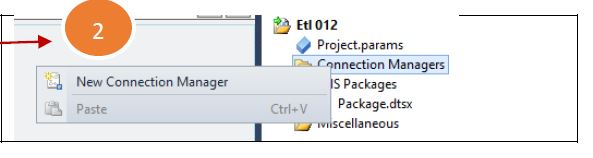
\includegraphics[width=12cm]{./Imagenes/111}
	\end{center}	

- Selección de OLEDB como Driver de Conexión BD

	\begin{center}
	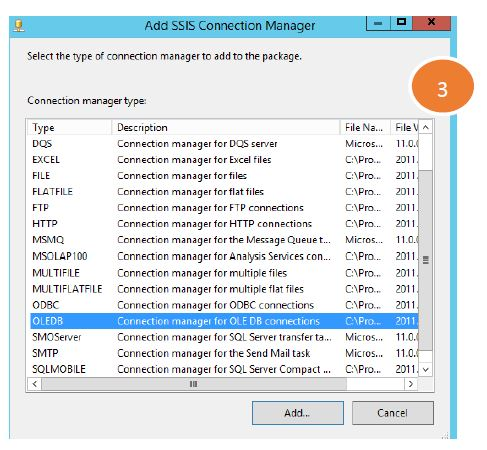
\includegraphics[width=13cm]{./Imagenes/12}
	\end{center}	

- Configuración de Conexión.

	\begin{center}
	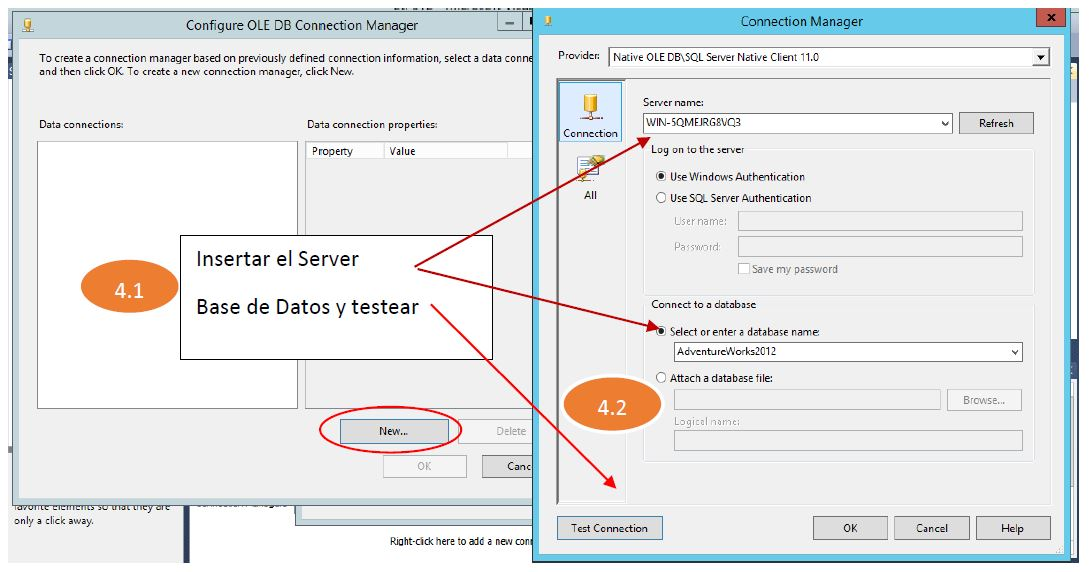
\includegraphics[width=17cm]{./Imagenes/13}
	\end{center}	

- Resultado de la Configuración.

	\begin{center}
	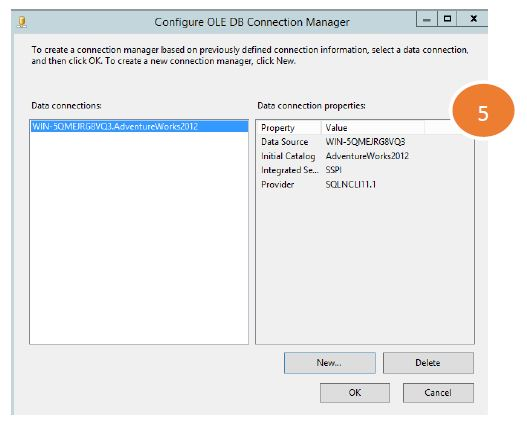
\includegraphics[width=14cm]{./Imagenes/14}
	\end{center}	

\begin{itemize}
    \item \textbf{Insertar: Execute SQL Task y Script Task}

	\begin{center}
	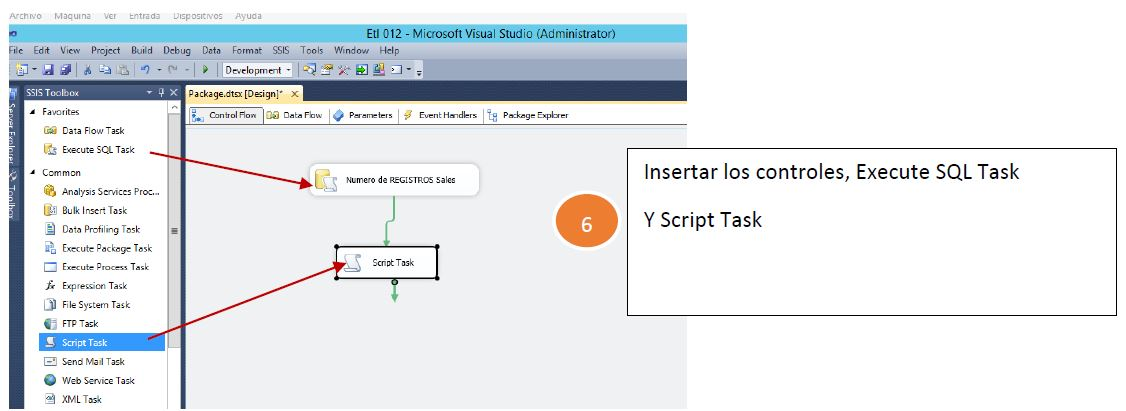
\includegraphics[width=17cm]{./Imagenes/15}
	\end{center}	

	\begin{center}
	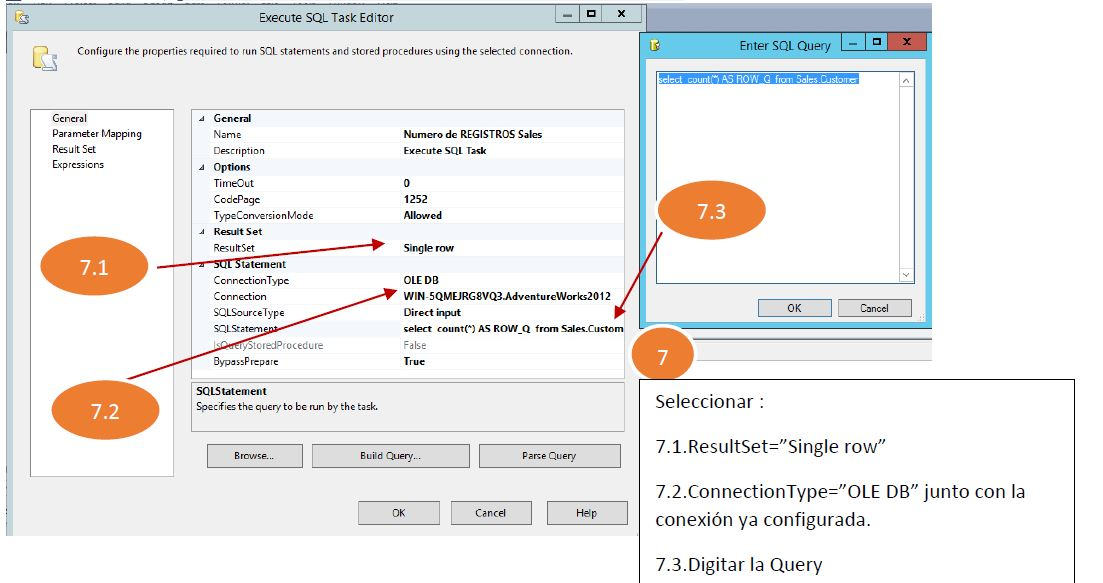
\includegraphics[width=17cm]{./Imagenes/16}
	\end{center}	

- Crear la Variable:

	\begin{center}
	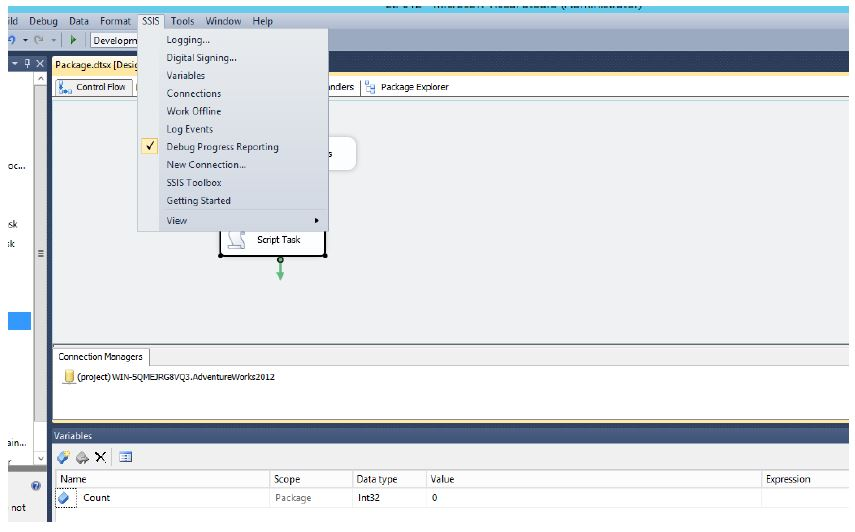
\includegraphics[width=15cm]{./Imagenes/17}
	\end{center}	

- Asignar la variable en “Numero de Registros Sales”.

	\begin{center}
	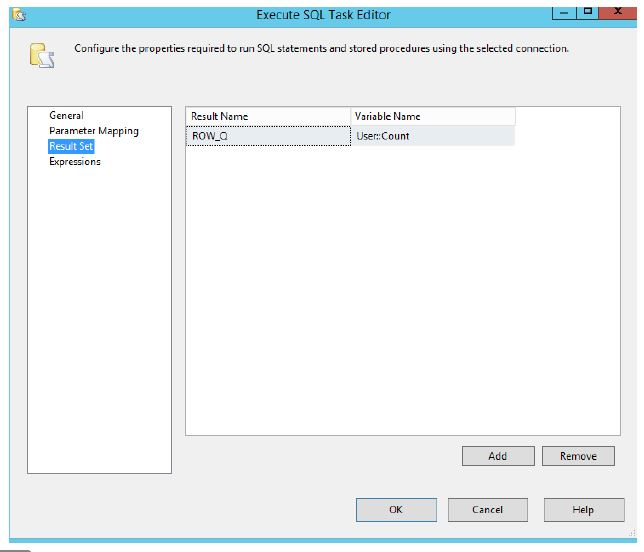
\includegraphics[width=13cm]{./Imagenes/18}
	\end{center}	

    \item \textbf{EDITAR COMPONENTE “Script Task Editor”}

	\begin{center}
	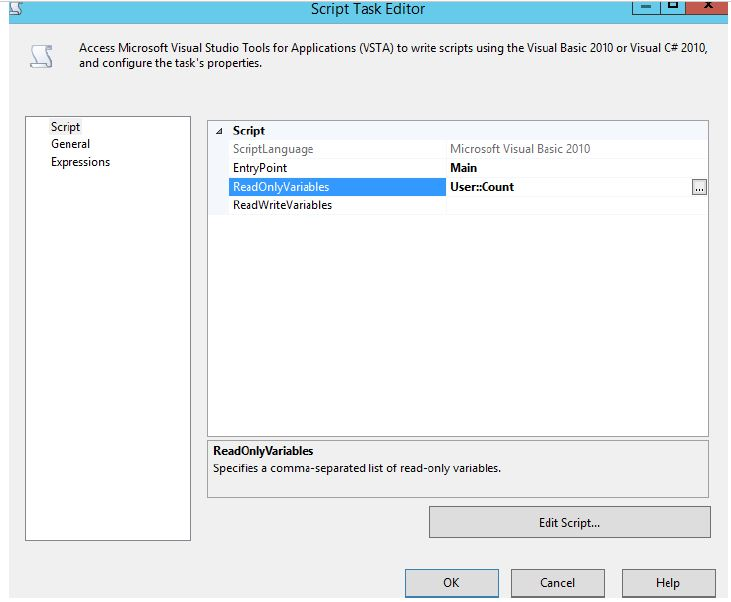
\includegraphics[width=13cm]{./Imagenes/19}
	\end{center}	

- Insertar este código “MsgBox(Dts.Variables(0).Value, MsgBoxStyle.Information)”

	\begin{center}
	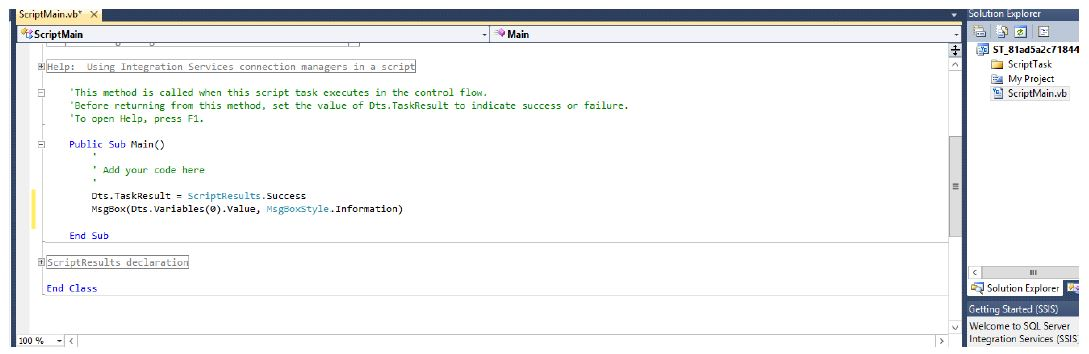
\includegraphics[width=17cm]{./Imagenes/20}
	\end{center}	

- Guardamos el proyecto y EJECUTAMOS Y LISTO.

	\begin{center}
	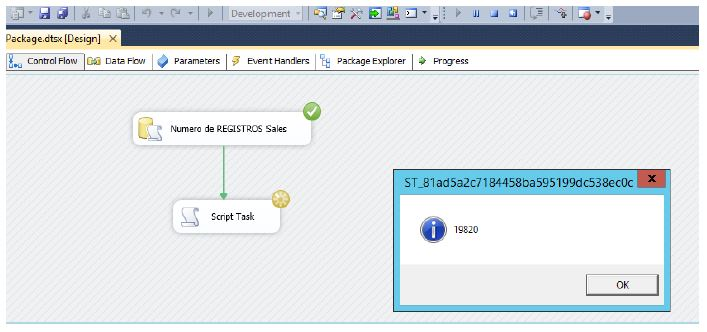
\includegraphics[width=15cm]{./Imagenes/21}
	\end{center}	
\end{itemize}
\section{CARGAR DATOS DE CLIENTES EN LA TABLA CUSTOMER DE BD ADVENTURE WORK} 

- Crear una nueva conexión para la base de datos AdventureWorksLT2012
- Crear un paquete nuevo Paquete.

	\begin{center}
	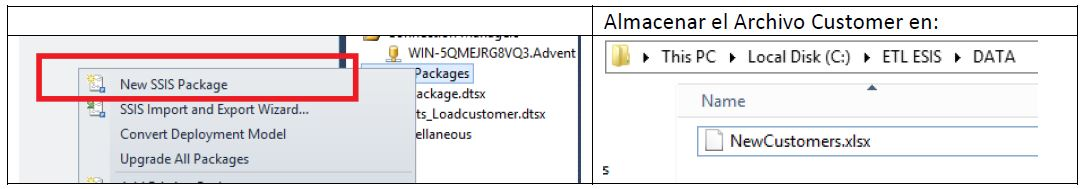
\includegraphics[width=13cm]{./Imagenes/22}
	\end{center}	

Este es el Diagrama Final que lo haremos Juntos en CLASE.

	\begin{center}
	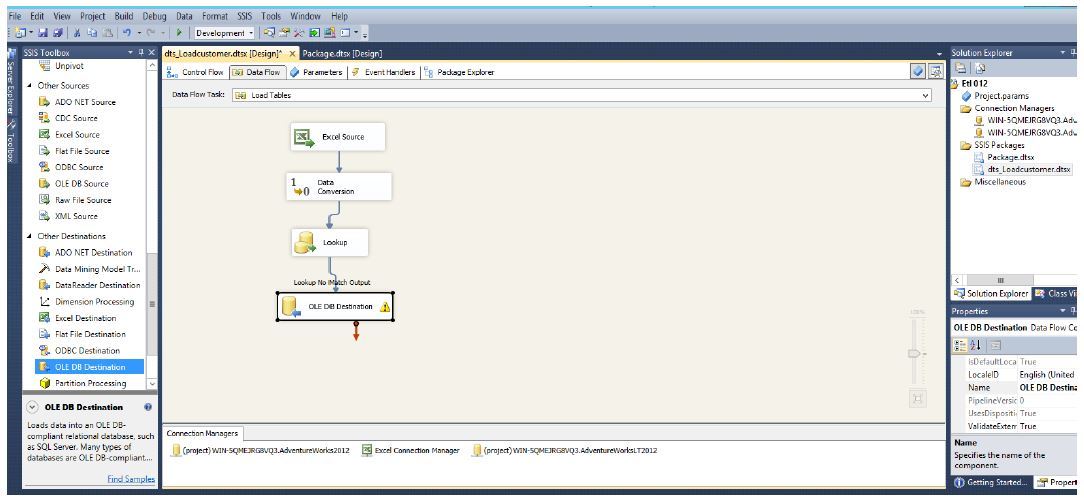
\includegraphics[width=17cm]{./Imagenes/23}
	\end{center}	

- Ejemplo: conexión con AdventureWork (INSERTAR DATOS EN UNA TABLA)

	\begin{center}
	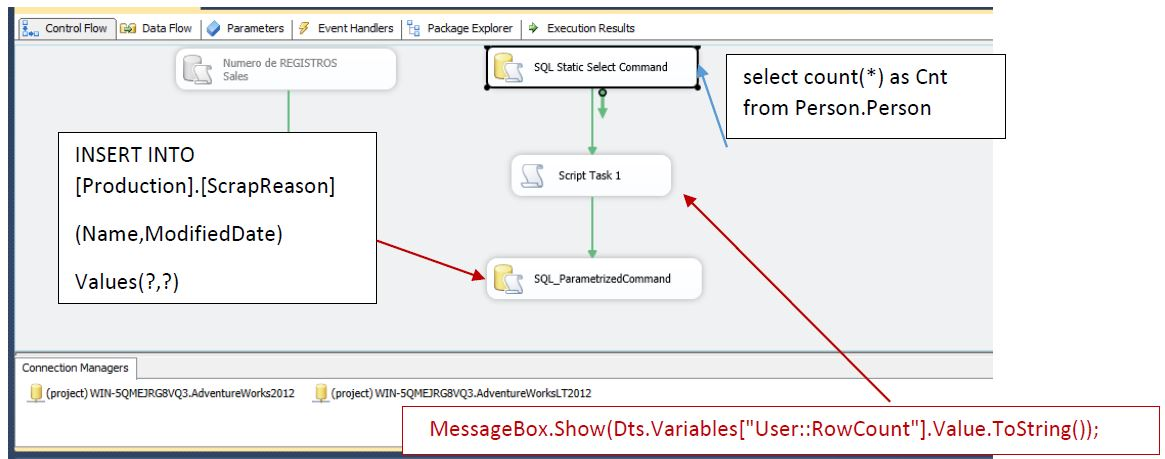
\includegraphics[width=17cm]{./Imagenes/24}
	\end{center}	

	\begin{center}
	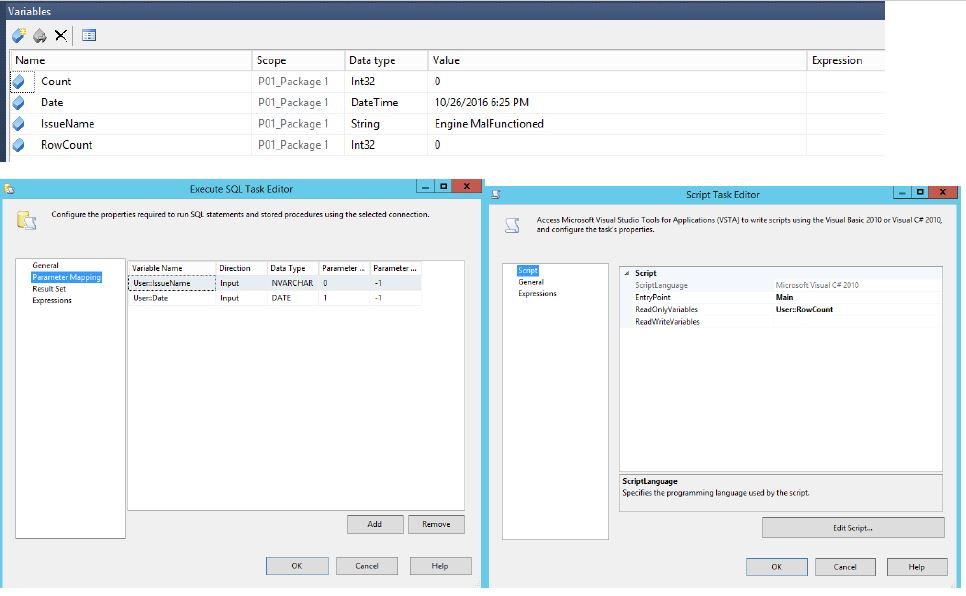
\includegraphics[width=17cm]{./Imagenes/25}
	\end{center}	
\section{TRABAJO ENCARGADO} 

EL Área de Marketing ha recolectado una lista de 1000 Clientes potenciales y 300 de ellos han comprado algunos de nuestros productos, y los vendedores lo han registrado en Excel, igual forma los registros en Excel de las ordenes y sus detalles de ventas.
El Gerente de Marketing quiere que sean cargados al Sistema en un tiempo corto de horas, Los técnicos siempre lo cargan usando la interface del sistema, y siempre demoran entre 3 dias y cometen ciertos errores al digitar.
y se ha vuelto costumbre que los técnicos lo hagan todo a mano.
Entonces el Gerente de Marketing recurre a Sector de TI para que ellos brinden alguna alternativa de procesamiento rápido, eficaz, y con un riesgo muy bajo de errores.
Se sabe que los vendedores que recolectan estos datos no siempre entregan todo bien Limpio, normalizado.
Marketing tiene asignado un directorio donde están copiando los archivos.

\begin{itemize}
    \item \textbf{GENERAR ARCHIVOS EN EXCEL PARA CUSTOMER y diseñar un ETL para la carga automática.}

En muchas oportunidades, en proyectos donde se tienen que trasladar archivos a un reporsitorio sea del usuario final o sea que el usuario deja compartido, y se tiene que procesar para cargarlo al sistema o aun Data Warehouse, en SSIS se cuenta con la funcionalidad de desarrollar esto.

ESTRUCTURA DE CONTROL FLOW: FUNCIONALIDAD (Manipulación, Mover, Renombrar el Archivo)

	\begin{center}
	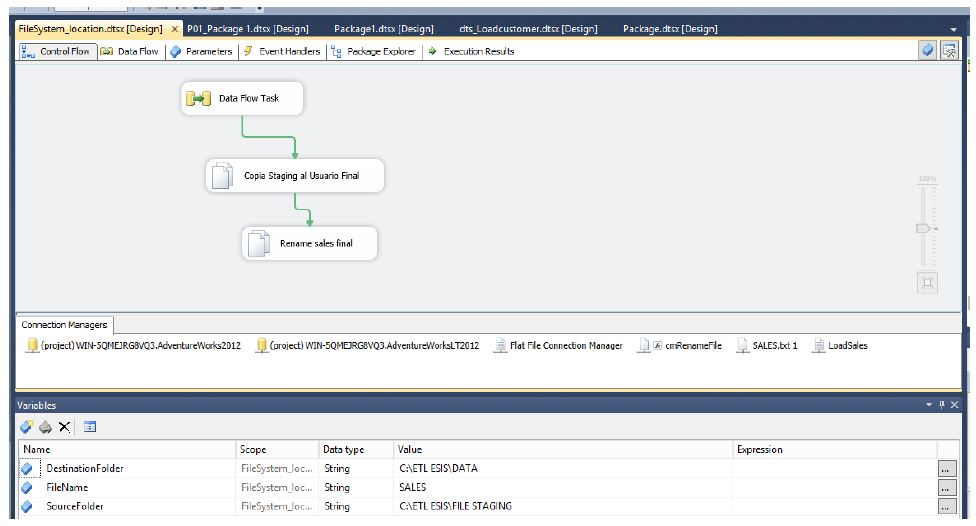
\includegraphics[width=17cm]{./Imagenes/26}
	\end{center}	

- Desarrollo de: Data Flow Task.

	\begin{center}
	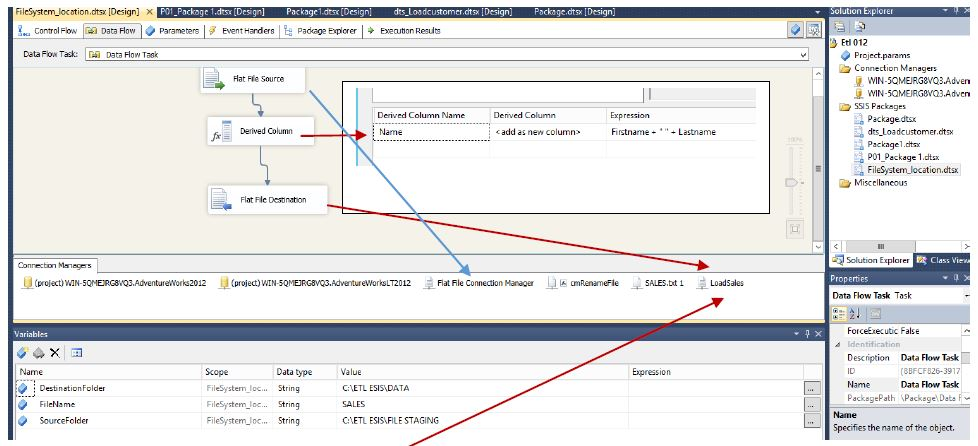
\includegraphics[width=17cm]{./Imagenes/27}
	\end{center}	

    \item \textbf{CREACION DE NEW FILE CONECCION}

	\begin{center}
	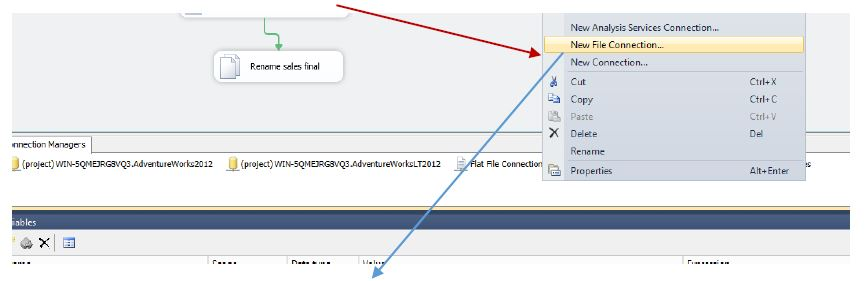
\includegraphics[width=17cm]{./Imagenes/28}
	\end{center}	

	\begin{center}
	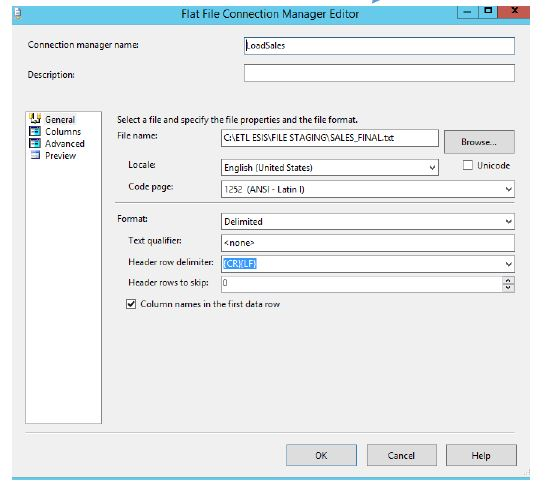
\includegraphics[width=14cm]{./Imagenes/29}
	\end{center}	

- Configuramos el Path de cmRenameFile. Usando expresiones y variables.

	\begin{center}
	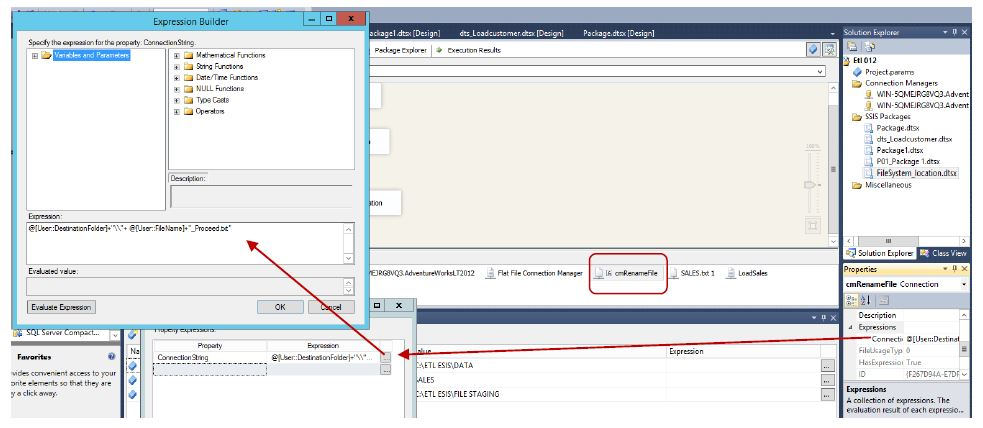
\includegraphics[width=17cm]{./Imagenes/30}
	\end{center}	

-Los procesos ETL deben ser capaz de copiar los archivos a su Espacio Staging para desde ahí realizar la carga al SSIS, Limpiarla y darle formato para cargarlo a la tabla objetivo.
\end{itemize}

\end{document}
